\documentclass[a4paper,11pt,oneside]{book}

% packages 
\usepackage{arsclassica}    % fancy layout
\usepackage[english]{babel}\addto{\captionsenglish}{\renewcommand{\bibname}{References}}
\usepackage{caption}         % figure captions
\usepackage[square,numbers,super,sort&compress]{natbib}  % bibliography style
\usepackage[cc]{titlepic}    % enable logo on title page
\usepackage{graphicx}       % logo related

\usepackage{bm} % bold math
\usepackage{amsmath} % underset
\usepackage{hyperref} % urls
\usepackage[]{algorithm2e}
\usepackage{array}
\usepackage{booktabs}

% Margins for pretty version ::
%\usepackage[pass]{geometry}
% Margins for university regulations ::
\usepackage[top=2cm, bottom=4cm, left=4cm, right=2.5cm]{geometry}
\usepackage{setspace}
\onehalfspacing

% don't hang captions
\captionsetup{format=plain}

\newcolumntype{L}{>{\centering\arraybackslash}m{4cm}}
\definecolor{light-gray}{gray}{0.95}

\usepackage{bm}
\DeclareMathOperator*{\argmin}{arg\,min}
\usepackage{tikz-cd}

\usepackage{standalone}
\standalonetrue 

% bibliography
\bibliographystyle{../thesis}

% title setup
\title{ \vspace{3in} Unravelling higher order genome organisation {\small [working
    title]} \\ \vspace{2em} {\large {\bf Methods section}} }
\author{Benjamin L. Moore}
\titlepic{\vspace{2.2in} 
\includegraphics[width=\textwidth]{/Users/benmoore/hvl/1yrReport/figs/igmm.png}}

\begin{document}

%\maketitle

\chapter{Methods}

\section{Hi-C data}\label{methods:hic}

\subsection{Mapping}\label{methods:mapping}

Raw Hi-C reads were downloaded from published datasets (Table \ref{hictable}) through
the Gene Expression Omnibus (GEO)\citep{Barrett2013} or the Short Read Archive (SRA)\citep{Leinonen2011a} with identifiers:
GSE35156 (H1 hESC), GSE18199 (K562) and SRX030113 (GM12878). These
paired reads were mapped independently to a reference genome: hg19/GRCh37 for human data, and mm10/GRCm38 for mouse. 

\begin{table}
\centering
\caption[Public Hi-C data used in this work.]{ {\bf Public Hi-C data used in this work.} }
\label{hictable}
\begin{tabular}{lllr}
{\bf Cell line} & {\bf Total reads} & {\bf Accession} & {\bf Citation}\\
\hline
Gm12878 & 31$\times10^{6}$ & \href{http://www.ncbi.nlm.nih.gov/sra/SRX030113[accn]}{SRX030113} & \citenum{Kalhor2012} \\
H1 hESC & 331$\times10^{6}$ & \href{http://www.ncbi.nlm.nih.gov/geo/query/acc.cgi?acc=GSE35156}{GSE35156} &\citenum{Dixon2012} \\
K562 & 36$\times10^{6}$ &  \href{http://www.ncbi.nlm.nih.gov/geo/query/acc.cgi?acc=GSE18199}{GSE18199}  & \citenum{Lieberman2009} \\
\hline
Cortex & 373$\times10^{6}$ & \href{http://www.ncbi.nlm.nih.gov/geo/query/acc.cgi?acc=GSE35156}{GSE35156}& \citenum{Dixon2012} \\
mESC & 476$\times10^{6}$ & \href{http://www.ncbi.nlm.nih.gov/geo/query/acc.cgi?acc=GSE35156}{GSE35156}&\citenum{Dixon2012} \\
\hline
IMR90 & 355$\times10^{6}$ &\href{http://www.ncbi.nlm.nih.gov/geo/query/acc.cgi?acc=GSE35156}{GSE35156} &\citenum{Dixon2012} 
\end{tabular}
\end{table}

Mapping was performed using the \texttt{hiclib} software
package\citep{Imakaev2012} and \texttt{bowtie2}\citep{Langmead2012} with
the \texttt{-{}-very-sensitive} flag. An iterative mapping approach was used to maximise the number of aligning fragments.\cite{Imakaev2012} Each fragment end was aligned first using short terminal sub-sequences. Those unmapped or with ambiguous mapping were then taken forward into the next iteration and extended until the entire fragment end had been aligned. Those remaining pairs with one or more unmapped ends were discarded.

This approach is designed to maximise uniquely-alignable fragment ends, while avoiding mismappings caused by crossing the fragment junction.\cite{Lajoie2014} 

\subsection{Filtering}\label{methods:filtering}

After mapping, interactions are first aggregated into restriction fragments then by regular binning of various resolutions (particularly 40 kb, 100 kb and 1 Mb). Several filters were applied at this stage, with the following cases removed:\cite{Imakaev2012, Lajoie2014} 
\begin{itemize}
\item Reads directly adjacent to a restriction enzyme site (within 5 bp)
\item Identical read pairs (presumed PCR duplicates)
\item Very large restriction fragments ($>100$ kb) which are likely from a repetitive or poorly-assembled region
\item Extremely over-represented fragments (top $.05\%$) which may throw-off eigenvector derivation
\end{itemize}

\subsection{Correction}\label{methods:correction}

Iterative correction and eigenvector expansion (ICE) is an approach to normalisation and processing Hi-C data, implemented as software library written in \texttt{python}.\citep{Imakaev2012} The iterative correction algorithm performs matrix balancing with the aim of generating a doubly stochastic matrix from raw interaction counts.\cite{Lajoie2014} That is, such that symmetric matrix $\mathbf{A}$ has both row and columns of equal sum. In practice, this effectively enforces "equal visibility" of each fragment, correcting for previously-described biases in interaction recovery such as GC-content and fragment length\cite{Yaffe2011} but without explicitly modelling these latent variables. This procedure is thus converting actual interaction counts into normalised interaction frequencies (IF), and to relative rather than absolute quantities. Scaling of IFs permits comparison of Hi-C experiments with very different sequencing depths (as is the case in this work, see Table \ref{hictable}). Despite differences in the levels of sequencing, otherwise the experiment methods underlying the produced Hi-C data were similar: the HindIII restriction enzyme was used in each case and the Hi-C protocol was largely unchanged (that is, we did not consider data from Hi-C variants such as TCC\cite{Kalhor2012} and \emph{in-situ} Hi-C\cite{Rao2014}).

\subsection{Eigenvector calculation}\label{sec:eigs}
Additional functionality provided by ICE is the eigenvector expansion of normalised contact maps. Eigenvectors from observed/expected matrices were chosen for consistency with Lieberman Aiden \emph{et al.},\cite{Lieberman2009} as opposed to the related eigenvectors calculated in Imakaev \emph{et al.}\cite{Imakaev2012} from the corrected maps alone. The details of this procedure are described in section \ref{sec:compartments}. Briefly, observed contacts (O) are divided by an expected matrix (E) which is generated by averaging the super- and sub-diagonals of the O matrix. That is, the E matrix gives the expected value of interactions at a given distance.

Importantly, the first two principle components (PCs) were calculated, and that with the highest absolute Spearman correlation with GC content is taken to reflect A/B compartmentalisation. PC eigenvectors were then orientated to positively correlate with GC, ensuring positive values reflected A compartments and negative values B compartments. Another subtlety is the calculation of eigenvectors per chromosome arm as opposed to per chromosome, this prevents issues with some meta- and submetacentric chromosomes where the first principle component indicated chromosome arms.\cite{Lieberman2009, Imakaev2012} Eigenvector expansion was performed on both 1 Mb and 100 kb matrices, below these resolutions results became less stable, and besides it has been shown that eigenvectors at higher resolution --- when they do indeed capture A/B compartmentalisation --- add little, if any, additional information.\cite{Fortin2015a}

\subsection{TAD calling}\label{meth:tadcalling}

TADs were called using the software provided in
\citet{Dixon2012} and their recommended parameters. This method is introduced in Section \ref{intro:tads} (see also Fig. \ref{fig:dicalc}) but will be described here in greater detail.

The TAD calling algorithm is a multi-stage process. Firstly, a statistic called the "directionality index" (DI) is calculated for each bin.\cite{Dixon2012} The equation for calculating the DI of a given bin is shown (Eqn. \ref{eqn:di}), where $U$ represents the sum of reads mapped up to $2$ Mb upstream of a given $40$ kb bin, and $D$ likewise for downstream contacts. Here $E$ is the expected number of downstream or upstream contacts (equal under the null hypothesis), hence is $E = \frac{U + D}{2}$. 

\begin{equation}\label{eqn:di}
\mathrm{DI} = \bigg(\frac{U - D}{|U - D|}\bigg)\bigg(\frac{(D - E)^2}{E} + \frac{(U - E)^2}{E}\bigg)
\end{equation}\vspace{.2em}

Equation \ref{eqn:di} can be intuitively understood as first determining the direction of the bias (the sign is given by $\frac{U - D}{|U - D|}$) and then calculating the extent of the bias (with $\frac{(D - E)^2}{E} + \frac{(U - E)^2}{E}$ being akin to a $\chi^2$-type statistic).\cite{Dixon2012}

This DI metric could be used as-is to call domains. Peaks of downstream contacts culminating in a peak of upstream contacts would delineate self-interacting domains. However, \citet{Dixon2012} instead use a hidden Markov model (HMM; Methods \ref{meth:hmm}) in a manner similar of that we later employed to call compartments (Section \ref{sec:compartments}). 

Here, the DI metric is considered a noisy observation emitted by an unobserved underlying three-state sequence of upstream, downstream or no- directional contact bias.\cite{Dixon2012} The HMM was fit to each chromosome with between 1 and 20 Gaussian mixtures allowed per state, however in some cases the expectation-maximisation (EM) algorithm used to parameterise these hidden states failed to converge; such cases were ignored. The Akaike information criterion (AIC) was used to selection the optimal number of mixtures (in practice, we found 5--10 were selected). 

Finally, given a fully-specified HMM we can calculate the posterior probability of a given state in a specific bin, using the forward-backward algorithm and given its observed data and preceding state sequence. \citet{Dixon2012} enforce the heuristic that regions are only classified as downstream- or upstream-biased if the state is called for two consecutive bins, or if a single bin has an especially high posterior probability ($\geq .99$). Domains are called from this state sequence and run from an initial downstream-biased bin through to the last in a run of $\geq 2$ of upstream biased states. This procedure was implemented by \citet{Dixon2012} in \texttt{Matlab}.

\section{ENCODE features}\label{methods:encode}

Genome-wide ChIP-seq datasets for: 22 DNA binding proteins and 10
histone marks were made available by the ENCODE
consortium\citep{Dunham2012, Boyle2014} along with DNase I
hypersensitivity and H2A.z occupancy, for each of the Tier 1 ENCODE cell
lines used in this work: H1 hESC, K562 and GM12878. These data were
pre-processed using MACSv2\citep{Zhang2008} to produce signal fold-change
relative to input chromatin. In most cases a paired input control was generated per cell type and by the same laboratory as that which performed a set of ChIP-seq experiments.\cite{Boyle2014} GC content was also calculated and used in
the featureset to give 35 total inputs (Table \ref{tab:features}).

\begin{table}[h]
\centering
\caption{ ChIP-seq and other public datasets used in this work. }
\label{tab:features}
\begin{tabular}{L | L | c} \toprule
\multicolumn{1}{m{4cm}}{\centering Histone modifications} &
\multicolumn{1}{m{4cm}}{\centering DNA binding proteins} &
\multicolumn{1}{m{2cm}}{\centering Other} \\
\midrule

% histone modifications
H3K27ac, 
H3K27me3, 
H3K36me3, 
H3K4me1, 
H3K4me2,  
H3K4me3, 
H3K79me2, 
H3K9ac, 
H3K9me3, 
H4K20me1 &

ATF3, CEBPB, CHD1, CHD2, CMYC, CTCF, EGR1, EZH2, GABP, JUND, MAX, MXI1, NRSF, POL2, P300, RAD21, SIX5, SP1, TAF1, TBP, YY1, ZNF143 &

\multicolumn{1}{m{2cm}}{\centering DNase, GC content, H2A.Z }\\

\end{tabular}
\end{table}

\subsection{Clustering input features}

To quantify collinearity of input features, correlation matrices built from genome-wide vectors of input feature measures were build and hierarchicaly clustered. The "significance" of observed clustering was assessed using sub- and super-sampled bootstrapping, with stable clusters deemed significant, as implemented in the \texttt{pvclust} R package.\cite{Suzuki2006a}

\section{Modelling compartment eigenvectors}\label{modelling}

\subsection{Random Forest}\label{sec:rf}

\begin{figure}
\begin{center}
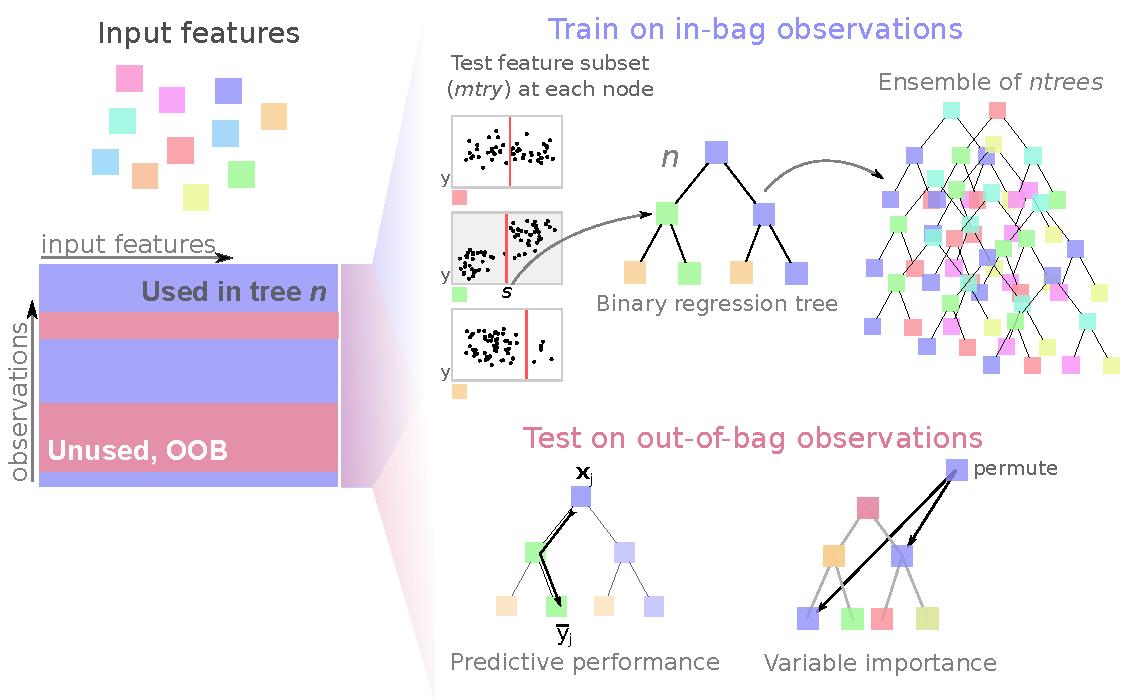
\includegraphics[width=4.5in]{figs/randforests.pdf}
\captionsetup{width=\textwidth}
\caption[Random Forests overview.]{ {\bf Random Forests overview. } 
 Random Forests are an ensemble of bagged, de-correlated classification or regression trees first described by Breiman.\cite{Breiman2001a}
}\label{fig:randforests}
\end{center}
\end{figure} 

Random Forest (RF) regression,\cite{Breiman2001a}  was used
as implemented in the R package \texttt{randomForest}.\cite{Liaw2002}
The RF algorithm (Fig. \ref{fig:randforests}) makes use of a collective of regression trees (size $ntrees$), each built from a
bootstrapped sample of the training set. In growing each tree, a small
number of variables ($mtry$) is tested at each bifurcation node, and that which minimises the
variance in child node subsets is selected at a specific
threshold. Having trained a group of trees, these can then be used as
predictive tools by inputting a vector of features to each tree and
averaging the output leaf node value across the forest. RF regression
was used as it is known to be one of the most powerful regression
methods developed to date,\cite{Svetnik2003, Cutler2007} typically
providing low bias and low variance predictions without the need for
variable selection.\cite{Diaz2006, Dasgupta2012}

Additionally the RF method represents an example of ``algorithmic
modelling''\cite{Breiman2001b} in that it makes no assumptions about the
underlying data model.
Parameters of $mtry = \frac{n}{3}$ (where $n$ is the number of input features) and $ntrees =
200$ were assumed as they are known to be
largely insensitive;\cite{Dasgupta2012, Hastie2001} this was verified
with the dataset used in this work (Fig. \ref{fig:rfparam}). 

\begin{figure}
\begin{center}
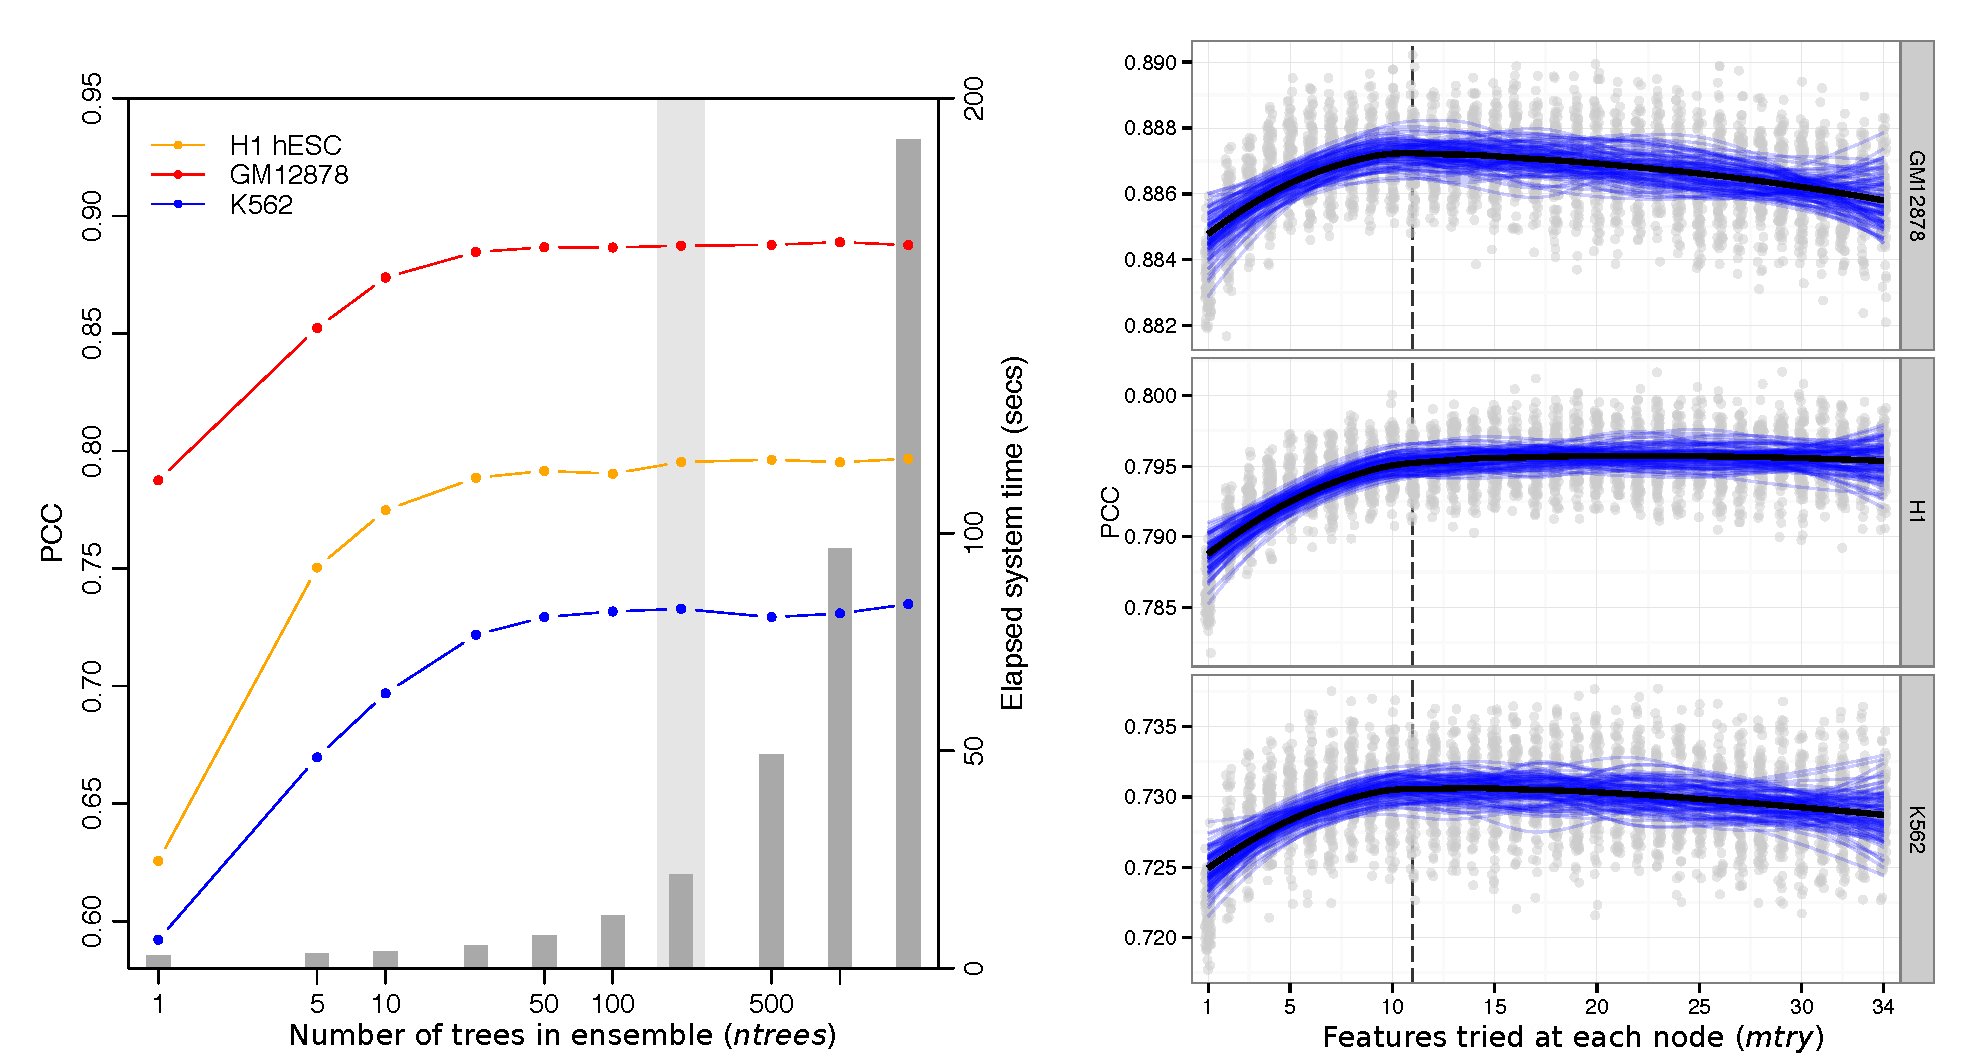
\includegraphics[width=5in]{figs/rfparams.pdf}
\captionsetup{width=\textwidth}
\caption[Random Forest parameters are largely insensitive.]{ {\bf Random Forest parameters are largely insensitive. } 
Two user-facing Random Forest paramters are known to be insensitive over a broad range.\cite{Hastie2001} Optimisations for $ntrees$ (the number of trees in the forests) and $mtry$ (the number of features tested at each node) are shown for three different models, with typical values of 200 trees and $\frac{1}{3}$ of input variables highlighted.
}\label{fig:rfparam}
\end{center}
\end{figure} 

Variable importance within Random Forest regression models was measured
using mean decrease in accuracy in the out-of-bag (OOB) sample. This
represents the average difference (over the forest) between the accuracy
of a tree with permuted and unpermuted versions of a given variable (Fig. \ref{fig:randforests}), in
units of mean squared error (MSE).\citep{Cutler2007, Dasgupta2012}

\subsection{Model performance}\label{sec:modelperf}

The effectiveness of the modelling approach was measured by four
different metrics. Prediction accuracy was assessed by the Pearson
correlation coefficient between the OOB predictions and observed eigenvectors, and the root mean-squared
error (RMSE) of the same data. Classification error, when predictions
where thresholded into $A \geq 0; B < 0$, was also calculated using
accuracy (\% correct classifications or True Positives) and area under
the receiver operating characteristic (AUROC) curve. Together these give
a comprehensive overview of the model performance, both in terms of
regression accuracy of the continuous eigenvector, and in how that same
model could be used to label discrete chromatin compartments.

For cross-application of cell type specific models, a single Random
Forest regression model was learned from all 1 Mb bins for a given cell
type. This was then used to predict all bins from each of the other two
cell types.

To test the sensitivity of the models to resolution, we also applied cell-type specific models learnt at 1 Mb resolution to input features binned at 100 kb. This was done by training a Random Forest regression model on all available 1 Mb bins in a given cell type, then applying that model to the prediction of all compartment eigenvectors derived at 100 kb. Model performance was then assessed as above, with the caveat that here the test set represents a higher-resolution window onto the original training set, therefore we might expect this to inflate the measures of generalisation error.

\subsection{Hidden Markov models}\label{meth:hmm}

Hidden Markov models (HMMs) are used both for calling TADs (Methods \ref{meth:tadcalling}) and for identifying chromosome compartments (Methods \ref{sec:compartments}, discussed in Section \ref{sec:compcalls}). Here we briefly introduce the HMM framework in general terms.

HMMs are widely used in computational biology, and have been called "the Legos of computational sequence analysis"\cite{Eddy2004} due to their wide applicability. HMMs provide a probabilistic modelling framework to explore any system that can be reduced to a 1D state sequence.\cite{Eddy1996, Rabiner1989} In the discrete case, each state in this sequence is capable of "emitting" one of a number of symbols, each with its own probability. In the continuous case, used in this work, instead a state has an associated emission distribution which can be a simple univariate Gaussian or a more complex mixture model. After an emission, each state has a number of "transition" probabilities, where the sequence can either change to another state or remain in the same state.

A typical representation of an HMM is shown in Equation \ref{eqn:hmm}, where hidden states ($\theta$) emit a sequence of observed states ($y$).\cite{Volg2005}

\begin{equation}\label{eqn:hmm}
\begin{tikzcd}[column sep=1.2pc]
\ldots \arrow{r} & y_{i-1} \arrow{r} & y_i \arrow{r} & y_{i+1} \arrow{r} & \ldots\\
\ldots \arrow{r} & \theta_{i-1} \arrow{r} \arrow{u} &
\theta_I \arrow{u} \arrow{r} & \theta_{i+1} \arrow{u} \arrow{r} & \ldots
\end{tikzcd}
\end{equation}

HMM state emission and transition parameters can be learned from an observation sequence via the Baum-Welch algorithm,\cite{Baum1970} a special case of the Expectation-Maximisation algorithm applied to HMMs. Following initialisation of transition and emission matrices (this can be random), the Baum-Welch algorithm first performs the $E$-step, calculating the expected number of transitions and emissions via a Forward-Backward procedure, then the $M$-step re-estimates transition and emission parameters based on these expected values. These two steps repeat until the HMM parameters converge to a local maxima.

Given a fully-specified HMM, the Viterbi algorithm can be applied to find the most probable state sequence given a sequence of observations.\cite{ryan1993viterbi} Using the notation of Equation \ref{eqn:hmm}, the Viterbi algorithm finds $\hat{\theta} = \mathrm{argmax}_\theta \Pr( y, \theta)$ using dynamic programming.\cite{Volg2005}

\subsection{Stepwise regression}\label{meth:stepregress}

% Expand, equations etc.
Stepwise regression is a form of model selection used with multiple regression. This simple approach starts with a complete model and serially remove and/or add variables, then calculate a metric (here we use the Bayesian information criterion, BIC) which weighs the the model likelihood against model complexity. This process is iterated until the metric reaches a (local) minimum, thus creating a more parsimonious model which retains predictive accuracy and should be less prone to overfitting. Stepwise regression also aids interpretation by selecting representative features from collinear clusters.\cite{Mantel1970} 

It should be noted that despite its continued widespread usage, several statistical issues have been identified with the stepwise procedure for model selection.\cite{Hurvich1990, Whittingham2006}

\subsection{LASSO}\label{meth:lasso}

The least absolute shrinkage and selection operator (LASSO) is a form of $\ell_1$ regularisation that penalises the sum of absolute values of standardised regression coefficients. By penalising absolute values and sums, rather than squared values as in $\ell_2$ regularisation (Ridge regression, for example), coefficients can be shrunk to $0$ thereby removing terms from the model. Thus the LASSO combines coefficient shrinkage of techniques like Ridge regression with a type of feature selection by promoting model sparsity.\cite{Tibshirani1994, Hastie2001}

Simply put, the LASSO minimises the sum of squared errors subject to a tuneable constraint on the sum total of absolute model coefficients. In equation form, we are fitting a simple linear model:

\begin{equation}
\begin{aligned}
\hat{y} = \beta_0 + \beta_1 x_1 + \beta_2 x_2 + \ldots + \beta_n x_n\\
\mathrm{or}~~\hat{y} = \bm{X}\bm{\beta} %(+ \bm{\epsilon})
\end{aligned}
\end{equation} \vspace{.2em}

We then wish to find that $\bm{\beta}$ which minimises $\sum_{j=1}^{n}(\hat{y}_j - y_j)^2$ while at the same time satisfying the inequality:

\begin{equation}\label{eqn:lassoineq}
\sum\limits_{i=1}^{p} |\beta_i| \leq c
\end{equation} \vspace{.2em}

Where here $c$ represents a tuneable parameter inversely proportional to the level of regularisation imposed on the model. It can be seen, for example, that of $c$ is set to the sum of the coefficients fit by ordinary least squares, the LASSO solution will be equivalent. Eqn. \ref{eqn:lassoineq} can be contrasted with Ridge regression, where the same in inequality instead constrains $\sum_{i=1}^{p} \beta_j^2$.

Formally, the LASSO problem has been expressed as:\cite{Hastie2001}

\begin{equation}\label{eqn:lassolagrangian}
\hat{\beta}^\mathrm{lasso} = \argmin_\beta \bigg\{ 
\frac{1}{2} \sum_{i=1}^N (y_i - \beta_0 - \sum_{j=i}^p x_{ij}\beta_j)^2 
+ \lambda \sum_{j=1}^p |\beta_j|
\bigg\}
\end{equation} \vspace{.2em}

This formulation introduces the $\lambda$ parameter as used in Section \ref{sec:lassoreg}. This parameter translates $\beta$ coefficients, such that larger values of $\lambda$ place stronger constraints on the coefficient total, thus encourage greater shrinkage and model sparsity (Eqn. \ref{eqn:lassolagrangian}).

In this thesis, we used the \texttt{glmnet} R package to fit LASSO models.\cite{glmnet1, glmnet2} In order to select $\lambda$, we use a $10$-fold cross-validation approach on a separate held-out training set. We chose that $\lambda$ which produced a mean cross-validated error within $1$ standard error of the minimum, thus favouring a sparser model than the global minimima.

\subsection{Other modelling approaches}\label{meth:othermodels}
 
Linear regression was used as a baseline for comparison with more complicated approaches such as Random Forest. If the same modelling accuracy could be achieved with simple multiple linear regression, this would be a faster and more interpretable modelling framework.

Partial least squares (PLS) regression was also used to model compartment profiles. PLS regression is well-suited to highly correlated inputs, employing a dimensionality reduction step to help address this redundancy, yet lacks the interpretability of a multiple linear regression. Similar to RF, PLS regression is aimed at building highly-predictive models rather than understanding singular relationships between a predictor and independent variable.\cite{Tobias1995} The \texttt{plsdepot} R implementation of PLS regression was used in this work.

% XX circle of correlations


\section{Variable regions}\label{variable-regions}

\subsection{Stratification by
variability}\label{sec:variable}

Median absolute deviation (MAD) was chosen as a robust measure of the
variability in a given 1 Mb block between the three primary cell types
used in this work: H1, K562 and GM12878. Blocks were ranked by this
measure and split into thirds that represented ``low'' variability (the
third of blocks with the lowest MAD), ``mid'' and ``high'' variability.
Each subgroup was then independently modelled using the
previously-described Random Forest approach.

``Flipped'' regions are those whose compartment state differs in one
cell type relative to the other two. For example, if a 1 Mb bin was
classified as ``open'' in H1 hESC and ``closed'' in both K562 and
GM12878, this is said to be a ``flipped'' compartment (to open).

\subsection{Chromatin state enrichment}\label{enhancer-enrichment}
%explanation of combined states: http://rohsdb.cmb.usc.edu/GBshape/cgi-bin/hgTables?db=hg19&hgta_group=regulation&hgta_track=wgEncodeAwgSegmentation&hgta_table=wgEncodeAwgSegmentationCombinedGm12878&hgta_doSchema=describe+table+schema

Chromatin state annotations used in this work were retrieved from the ChromHMM\cite{Ernst2011} and SegWay\cite{Hoffman2012} combined annotations.\cite{Hoffman2013} These represent the consensus from two independent chromatin state prediction algorithms, and ignore regions of apparent disagreement; hence in theory making more robust and conservative predictions than either algorithm independently. Nevertheless, Hoffman \emph{et al.} caution that in areas of disagreement, each algorithm may highlight differing biological phenomena so should also be considered separately.\cite{Hoffman2013}

The set of state predictions from the combined algorithms are:
\begin{enumerate}
\item Predicted transcription start sites (TSS)
\item Promoter flanking regions
\item Transcribed reigons
\item Repressed regions
\item Predicted enhancers
\item Predicted weak enhancer or \emph{cis} regulatory element
\item CTCF-enriched elements
\end{enumerate}

Short, discrete state predictions such as enhancers were
considered ``shared'' if there was an overlapping enhancer annotation in
either of the two other cell types, and labelled as ``tissue-specific''
otherwise. This was repeated for each of the called chromatin states.

\subsection{Gene ontology analysis}

Variable regions (section \ref{sec:variable}) were tested for functional enrichments using Gene Ontology (GO) annotations.\cite{Ashburner2000} The DAVID tool\cite{Huang2008} was used to compare GO terms for genes located in variable compartments with a background set of genes within all annotated compartments.


\section{Boundaries}\label{boundaries}

\subsection{TAD boundaries}\label{meth:tadbounds}

Having called TADs (Section \ref{meth:tadcalling}), we then have a set of boundaries at the start and end of each domain. We generated average boundary enrichment or depletion profiles by averaging input features into 50 kb bins spanning $\pm450$ kb from the boundary bin.

To test for the enrichment or depletion of a chromatin feature over a
given boundary, a two tailed Mann-Whitney test was used to compare the
boundary bin with the ten outermost bins of the window (5 from either
side). The significance level at $\alpha = 0.01$ was then
Bonferonni-adjusted for multiple testing correction, and results with
\emph{p}-values exceeding this threshold were deemed significantly
enriched or depleted at a given boundary.

To compare boundaries between cells, each TAD boundary called in K562 and GM12878 were compared with those called in H1 hESC. For each boundary, the minimum absolute difference to the nearest matching boundary in H1 hESC was recorded, and this was then compared with a null model of an equal number of boundaries randomly-placed along available bins. A Kolmogorov-Smirnov test was then used to compare the empirical cumulative distributions of these distances.

\subsection{Compartments}\label{sec:compartments}

Eigenvectors were calculated as described in section \ref{sec:eigs}. A/B compartmentalisation has previously been called simply from the properly-orientated principle component eigenvector, with positive values representing a bin in an A compartment state, and negative values representing a bin in a B, more repressive state.\cite{Lieberman2009} 

Compartment boundaries were called by first training a two-state hidden
Markov model (HMM) on the compartment eigenvector and then using the
Viterbi algorithm to predict the most likely state sequence that
produced the observed values (Methods \ref{meth:hmm}). Justification for this approach is discussed in Section \ref{sec:compcalls} and we also note the similar use of an HMM in TAD calling (Section \ref{meth:tadcalling}).

%HMM states distribution plots

The point at which transitions occurred
between states was taken as a boundary which was then extended $\pm 1.5$~Mb to give a $3$~Mb window in which a boundary was though to occur. Boundary enrichments and alignments were tested in the same manner as TADs (Section \ref{meth:tadbounds}).


\section{Predicting TAD boundaries}\label{meth:tadpred}

\subsection{AUC-RF}
% AUC_RF alorithm
% AUROC  why good
% Classification RF + gini coefficient

To predict TAD boundaries we used a classification Random Forest model, built with the AUC-RF algorithm,\cite{Calle2011} as implemented in the \texttt{AUCRF} R package. This is a form of stepwise model selection which optimises feature subset selection relative to the area under the receiver operating characteristic (AUROC), a metric which captures both the speciality and sensitivity of a classifier hence is better-suited to unbalanced datasets than previously-described RF variable selection methods that used simple classification accuracy.\cite{Diaz2006, Chen2012} The AUC-RF procedure has been successfully applied in other bioinformatics applications, such as identifying a subset of most relevant variants in a genome-wide association study.\cite{DeMaturana2013} 

More specifically, the AUC-RF algorithm is a backwards elimination procedure, commencing with variable ranking by importance. In these classification RF models, mean decrease in Gini impurity (Methods \ref{meth:gini}) was chosen as the measure of variable importance, as it proved to be more stable than mean decrease in accuracy on permuted data.\cite{Calle2011} Regardless, impurity and permutation-based importance measures are thought to be largely consistent in many cases.\cite{Liaw2002, Hastie2001}

Steps in the algorithm can be summarised as:\cite{Calle2011}
\begin{enumerate}
\item Train an RF classifier using all available variables and calculate variable importance
\item Remove the least important $10\%$ of variables and fit a new RF model
\item Calculate the AUROC on predictions made with out-of-bag data
\item Iterate steps 2--3 until a single variable model is built
\item Select that model with the highest AUROC
\end{enumerate} \vspace{.1em}

Importantly, AUC-RF avoids some of the problems of stepwise regression. Both over-optimistic model performance (due to repeated training and testing on the same pool of data) and errors due to the instability of variable rankings are mediated through an additional cross-validation step.\cite{Calle2011}

The input feature set for this model was made up of the same $35$ ENCODE features used in models of compartment eigenvector (Methods \ref{methods:encode}), with the addition of counts of Alu repeat elements (as used in Section \ref{sec:repeats}). TAD boundary bins were called as previously described (Methods \ref{meth:tadcalling}) and were resolved to 40 kb. Bins containing a TAD boundary were our true positives (TP), and to generate true negatives (TN) we took matched bins $450$ kb upstream of each boundary bin. Of these, a randomly-selected $80\%$ of TP/TN pairs were used as our training and validation set in each cell type, while the remaining $20\%$ of cases were held-out as independent test sets.

\subsection{Gini importance}\label{meth:gini}

The Gini impurity, $G$, of a single node containing some proportions of $n$ classes of variable is calculated as shown (Eqn. \ref{eqn:gini}), and is observably related to the concept of entropy or information gain. 

\begin{equation}\label{eqn:gini}
G = \sum_{i=1}^{n} p_i(1-p_i)
\end{equation}

In our simple two-class setting (i.e. boundary, $b$, or non-boundary), this simplifies to Equation \ref{eqn:ginisimp}. Here it can be seen that a $G$ of 0.5 means the node contains a $50:50$ split of class labels, whereas a node of $95\%$ boundaries has a much lower impurity ($G = 0.095$).

\begin{equation}\label{eqn:ginisimp}
G =  2p_{b} (1-p_{b})
\end{equation}

To convert the impurity into a measure of importance, we compare $G$ of a parent node with that of its two daughter nodes ($G_{d_1}$ and $G_{d_2}$), following a partition on a given variable of interest. %This decrease in Gini impurity can then be averaged over all splits in which a specific variable has been selected ($N_{used}$). This approach is described in Equation \ref{eqn:giniimportance}.

% text from ?importance :: The second measure is the total decrease in node impurities from splitting on the variable, averaged over all trees. For classification, the node impurity is measured by the Gini index. For regression, it is measured by residual sum of squares.
This decrease in Gini impurity can then be summed over all splits in which a specific variable has been selected per tree ($N_{used}$), and the averaged over all trees in the forest ($ntrees$). This approach is described in Equation \ref{eqn:giniimportance}.

% j = node; N_used : number of times var used; d_x = daughter
%\begin{equation}\label{eqn:giniimportance}
%I = \frac{1}{N_{used}} \sum_{j=1}^{N_{used}} G_{j} - (G_{d_1} + G_{d_2})
%\end{equation}

% actually looks like Gini is summed per tree, averaged per forest
\begin{equation}\label{eqn:giniimportance}
I = \frac{1}{ntrees} \sum_{ntrees} \sum_{j=1}^{N_{used}} G_{j} - (G_{d_1} + G_{d_2})
\end{equation}


\section{MetaTAD analysis}\label{meth:meta}

MetaTADs are a conceptual level of genome organisation discovered by collaborators in the Pombo lab. Their method for calling metaTADs involve the constrained hierarchical clustering of those neighbouring TADs with the greatest inter-TAD contacts. This pairing was recursed up to the level of whole chromosomes, thus resulting in a tree of increasing metaTAD aggregation. 

%Additionally our collaborators used an altered TAD calling method to that of \citet{Dixon2012} They used the directionality index (DI), as described in Section \ref{meth:tadcalling}), but replaced the subsequent steps with a simple thresholding method: when the DI crossed a threshold of standard deviation, $\sigma$, it was considered either an up- or downstream biased bin and TADs were called between

% expand XX

\subsection{Size selection}\label{sec:metatad}

For boundary analysis of metaTADs, again a similar approach was used to that of TADs (Section \ref{meth:tadbounds}) but thresholded to within a given range of sizes. MetaTADs below 10 Mb were excluded, as to have no lower bound results in $\frac{2}{3}$ of all TAD boundaries likewise considered MetaTAD boundaries, reducing the power to analyse any differences. 10 Mb was chosen in an attempt to compromise minimising the overlap between TAD and metaTAD boundaries, while also retaining a large enough sample size. An upper bound of 40 Mb was also chosen, as beyond this threshold inter-TAD contacts were found to be no higher than expected by chance. In practice, the tree-like structure means any upper-bound has little impact as a filter: in almost all cases, any boundary in a metaTAD of size $> 40$ Mb will also fortpalam metaTADs below this value. Additionally, the hierarchical nature of metaTADs means that some boundaries are present at multiple levels of the tree. Only one case of each boundary position was tested for feature enrichments, and this was performed as with TAD boundaries (Section \ref{meth:tadbounds}).

\subsection{Collaborator datasets}\label{meth:metadata}
%CAGE, ctss
Our collaborators in the metaTAD project performed ChIP-seq experiments for PolIII (three variants), H$3$K$27$me$3$, CTCF and DNase-I hypersensitivity. Mapped reads from these experiments were processed using MACSv2\cite{Zhang2008} to give relative signal over background (from an estimated local model), which was then averaged over all boundaries genome wide. 

Cap analysis of gene expression (CAGE) data was produced by the FANTOM consortium.\cite{fantom5, itoh2012a} This method produces sequencing data from the $5`$ end of cDNAs, and can be used to quantify expression activity at precise promoter locations.\cite{Kodzius2006} Here, CAGE was performed at multiple points along a neural-differentiation timecourse and tags were clustered to form CAGE TSS (CTSS) in a manner developed for the FANTOM5 project.\cite{fantom5} To count these CTSS over boundary bins, we simply intersect the annotations and count CTSS per bin using \texttt{bedtools}.\cite{Quinlan2010}

Gene density over metaTAD boundaries was calculated using UCSC \texttt{mm9} gene models.\cite{Karolchik2014} Again simple intersections were taken to count genes over boundaries using \texttt{bedtools}\cite{Quinlan2010} and requiring a minimal overlap fraction of $0.5\%$ of a bin ($250$ bp).

\subsection{LAD coincidence}\label{meth:metalad}

To compare metaTAD boundaries with those of LADs, we made use of previously-published Lamin-B1 DamID microarray probe intensities.\citet{Peric-Hupkes2010} For analysis over boundaries, these values were averaged into the same boundary windows as used previously (50 kb bins $\pm450$ kb around boundary, as in Section \ref{meth:tadbounds}). 

Transitions between high and low lamina association were detected by fitting a linear regression model across each series of consecutive boundary bins (i.e. $\textrm{Lamina assoc.}=\beta\cdot\textrm{bin} + c$). Linear models which had an absolute coefficient $|\beta| >.05$ were taken as crossing a LAD transition. This threshold is a heuristic which appears to perform well at conservatively selecting clear transitions. As a method of seriation for the $y$-axis of heatmap figures (e.g. Fig. \ref{fig:mtlamin}), boundaries were divided into those that coincided with a lamin transition and those that did not, and members within each group were then sorted by average intensity. 

To test the significance of the association between boundaries and lamin transitions, we circularly permuted both TAD and metaTAD boundaries on each chromosome 1000 times, and calculated the proportion of boundaries that crossed LAD boundaries using the same linear regression procedure described above. Empirical $p$-values were then calculated as the number of permuted results greater than or equal to the observed value.

\section{Giemsa band comparison}\label{giemsa-band-comparison}

Cytogenic band data and Giemsa stain results were downloaded from the
UCSC genome browser (table \texttt{cytoBandIdeo}). The genomic
co-ordinates are an approximation of cytogenic band data inferred from a
large number of FISH experiments.\citep{Furey2003}

To compare G-band boundaries with our compartment data, we allowed for a
$\pm 500$ kb inaccuracy in G-band boundary. For each G-band boundary,
the minimum absolute distance to any compartment or TAD boundary was
calculated for each cell type. To generate a null model, \ldots

\section{Nuclear positioning}\label{methods:positioning}
Previously published data  on chromosome positioning preference within
the nucleus was used to label each chromosome as ``inner'', ``middle''
or ``outer''.\cite{Boyle2001} Chromosomes whose DAPI hybridisation
signals were significantly enriched ($p\leq 2\times10^{-2}$) in the inner nuclear shell, as
defined by Boyle \emph{et al.}\cite{Boyle2001}, made up the ``inner''
group and included chromosomes 1 and 16. Similarly the ``outer'' group
had enriched signals ($p\leq 5\times10^{-3}$) in the outer shell relative to the inner nuclear
shell and included chromosomes 2, 3, 11-13 and 18. The remaining
chromosomes in our filtered dataset, 6, 14 and 15, were assigned to
the ``middle'' group and showed no significant to either inner or
outer nuclear shells ($p \geq 0.1$).\cite{Boyle2001} The significance
of the difference in distribution of eigenvectors in the inner
versus outer shell was determined by a two-sided Kolmogorov-Smirnov (K-S)
test, with the alternative hypothesis that the empirical cumulative
density function of the inner chromosome eigenvectors $F_{inner}$ was not equal to $F_{outer}$. This chromosomal positioning data was measured in lymphoblastoid
cells though nuclear architecture is though to be largely conserved
between cell types\cite{Chambers2013, DeWit2013} and even higher primates,\cite{Tanabe2002} so should be comparable in this instance.

\section{Modelling transcriptional output}

\subsection{Reproducing a published study}\label{meth:dong}
In Section \ref{sec:reprodong} we reproduce and extend a previously published study by \citet{Dong2012}. In doing so, we reuse much of the code and materials made available by the authors and more widely the ENCODE consortium\cite{Dunham2012}, of which this paper was a part. Some scripts were extracted from the ENCODE virtual machine, designed to provide an environment in which to reproduce their main findings.\cite{Myers2011}

Input features for models of transcription were derived from the January 2011 ENCODE data freeze.\cite{Dunham2012} Normalised ChIP-seq signals were generated by ENCODE using \texttt{wiggler} and retrieved for this study as \texttt{bigWig} files. These were averaged into $40 \times 100$ bp bins across each GENCODE v7 TSS, to give $\pm 2$ kb windows around each start site. These bins were then used to find the `bestbin`, that which correlates best with transcriptional output on a training subset of TSS. A bin representing the average intensity over the whole gene (TSS to TES) was also considered. That which best correlated on a training set was then used as the representative region for that feature in subsequent modelling steps.\cite{Dong2012} The justification for this approach is discussed in Section \ref{sec:dongbestbin}.

\subsection{Predicting FANTOM5 data}\label{meth:fantom5}

We transferred this transcriptional modelling approach to what was at the time novel, unpublished CAGE data produced by the FANTOM consortium. This data has since been released in the FANTOM5 series of publications.\cite{fantom5}

We used H1 hESC $t_0$ CAGE data from a differentiation timecourse study, as generated by FANTOM5 members. The consortium pre-processed raw CAGE tags into clusters using decomposition-based peak identification.\cite{fantom5} To filter for gene-associated CAGE clusters, we discarded those tag clusters centered on a point $>50$ bp from an Ensembl (\texttt{v69}) annotated TSS, thereby removing enhancers and other non-genic transcribed regions. When multiple clusters were linked to the same TSS, that with the highest peak was kept. Expression was matched with ENCODE ChIP-seq data for the H1 hESC cell type (processed as described in Section \ref{meth:dong}) and an additional measure of replication timing. 

Input data for models of FANTOM5 CAGE are shown in Table \ref{tab:fantommodel}.

\begin{table}[h]
\centering
\caption{ ENCODE datasets generated in the H1 hESC cell line and used in models of transcriptional output. }
\label{tab:fantommodel}
\begin{tabular}{L |  c} \toprule
\multicolumn{1}{m{4cm}}{\centering Histone modifications} &
\multicolumn{1}{m{2cm}}{\centering Other} \\
\midrule

% histone modifications
H3K27ac, 
H3K27me3, 
H3K36me3, 
H3K4me1, 
H3K4me2,  
H3K4me3, 
H3K79me2, 
H3K9ac, 
H3K9me3, 
H4K20me1 &

\multicolumn{1}{m{2cm}}{\centering HDAC6, DNase I, H2A.Z, Input }\\

\end{tabular}
\end{table}

\section{4C analysis}\label{methods:4c}

For computational analysis of 3C-seq data (also known as 4C), the experimental protocol used by our collaborators recommends the \texttt{r3Cseq} R package,\cite{Stadhouders2013, Thongjuea2013} part of the BioConductor repository\cite{Gentleman2004, Huber2015} for the R programming environment.\cite{Ihaka1996}

This package produces normalised interaction frequencies which are comparable between experiments and then assigns statistical significance to any identified contacts, thereby reporting regions that co-localise to a greater degree than expected by their genomic proximity alone.

\subsection{Normalisation}\label{methods:4cnorm}

The normalisation procedure for 4C data is adapted from a previous method for normalising deepCAGE data between samples.\cite{Balwierz2009} In short, the reverse-cumulative distribution of read counts per restriction fragment is fit to a power-law model; this effectively encodes the \emph{a priori} expectation of exponential decay of the number of contacts as distance increases from the viewpoint. Transformed read counts per million (RPM) can then be retrieved from a standardised reverse cumulative distribution, parametrised with the empirical coefficient, $\alpha = -1.35$.\cite{Thongjuea2013}

This normalisation procedure has the effect of making the output RPM value independent of the original experiment's sequencing depth and, more importantly, acts to reduces the impact of artefacts and errors by enforcing the expected power-law relationship of restriction fragment read counts.

\subsection{Significance estimation}\label{methods:4csignif}

The \texttt{r3Cseq} package\cite{Thongjuea2013} also attempts to assign a measure of significance to observed contact frequencies. This is done through a simple method of background estimation based on observed values. The justification for this non-independent estimate of background signal is that a relatively small proportion of observed contacts are expected to be significantly enriched, thus won't unduly perturb an average signal.\cite{Thongjuea2013} An improved method that avoids this assumption has since been developed where a background model was iteratively fitted, with outlier removal at each revision.\cite{Ay2014}

Here a non-parametric cubic smooth spline is fit to normalised read count data using a heuristic smoothing parameter. This model then provides an expected level of interaction at a given distance from the viewpoint in \emph{cis}. From this, it is simple to calculate a $Z$--score as:

\begin{equation}\label{form:r3cseq}
Z = \frac{(O-E)}{\sigma}
\end{equation}

\noindent Where $\sigma$ is the standard deviation of residuals from the observed ($O$), expected ($E$) difference. This $Z$-score can then be converted to a $p$-value which in turn is corrected for multiple testing using bootstrapped estimates of false-discovery rate (FDR) $q$-values\cite{Storey2004} (as implemented in the \texttt{qvalue} R package\cite{qvalue}). This $Z$--test approach assumes a normally-distributed test statistic, an assumption that typically does not hold on 4C data where interactions distal to the viewpoint are increasingly sparse, however this approach and variants thereof have been applied in a variety 4C and 5C analyses (e.g. \citenum{Simonis2006, Sanyal2012, Splinter2012, Gao2013, Dixon2015, Crane2015}). Some publications (e.g. \citenum{Nora2012}) use a more appropriate distribution to assign $p$-values to the $Z$ statistic, such as the Weibull (extreme value) distribution.

While we are mostly concerned with these \emph{cis} interactions, \texttt{r3Cseq} also offers significance testing for \emph{trans} interactions between the viewpoint and restriction fragments on different chromosomes. Here instead of distance scaling, the expected ($E$) terms in Equation \ref{form:r3cseq} are genome-wide averages excluding regions $\pm$ 100 kb around the viewpoint.\cite{Thongjuea2013} This means the absolute values of normalised RPMs reported for \emph{trans} interactions are in practice upscaled, being equivalent to experimental RPMs less the most deeply-sequenced regions, i.e. the viewpoint and immediately adjacent regions.

\subsection{3--D modelling}\label{methods:3dmodelling}

\section{5C analysis}\label{methods:5c}

\section{Scripts and other analyses}

Much of this work has been performed by writing custom scripts in the R programming language.\cite{Ihaka1996} Code for the majority of analyses described in this thesis are available through a public git repository hosted on \texttt{github} at \href{https://github.com/blmoore/3dgenome}{github.com/blmoore/3dgenome} (instructions on how to reproduce analyses and figures are included therein). A special mention goes to the packages of Hadley Wickham which are used throughout, especially \texttt{ggplot2}\cite{ggplot2} and \texttt{dplyr}\cite{dplyr}.

The programming language python\cite{rossum1995} was also employed to a lesser-extent, as were command--line tools such as \texttt{bedtools}\cite{Quinlan2010} and \texttt{SAMtools}\cite{Li2009}. Additionally command-line \texttt{BigWig*} tools\cite{Kent2010} were used, as well as the UCSC genome browser associated data tracks.\cite{Kent2002, Raney2014, Kuhn2013a}.

\ifstandalone
\begin{small}
\bibliography{/Users/benmoore/Documents/library,/Users/benmoore/Documents/customrefs}
\end{small}
\fi

\end{document}
